\documentclass[brudnopis]{xmgr}
\usepackage{graphicx}
\graphicspath{ {images/} }
% Jeśli nowe rozdziały mają się zaczynać na stronach
% nieparzystych:
%\documentclass[openright]{xmgr}

%\defaultfontfeatures{Scale=MatchLowercase}
%\setmainfont[Numbers=OldStyle,Ligatures=TeX]{Minion Pro}
%\setsansfont[Numbers=OldStyle,Ligatures=TeX]{Myriad Pro}
% for fontspec version < 2.0
\setmainfont[Numbers=OldStyle,Mapping=tex-text]{Arial}
\setsansfont[Numbers=OldStyle,Mapping=tex-text]{Arial}
%\setmonofont[Scale=0.75]{Monaco}

% Opcjonalnie identyfikator dokumentu
% drukowany tylko z włączoną opcją 'brudnopis':
\wersja   {wersja wstępna [\ymdtoday]}

\author   {Michał Lipiński}
\nralbumu {105229}
\email    {michal@twoj.cloud}

\author   {Mariusz Piątek}
\nralbumu {205176}
\email    {mariusz.piatek92@gmail.com}

\author   {Paweł Ponieważ}
\nralbumu {228254}
\email    {p.poniewaz@o2.pl}

\title    {Dom Przyszłości w kontekście Internetu rzeczy}
\date     {2016}
\miejsce  {Gdańsk}

\opiekun  {dr Włodzimierz Bzyl}

% dodatkowe polecenia
%\renewcommand{\filename}[1]{\texttt{#1}}
%\definecolor{stress}{cmyk}{0,1,0.13,0} % RubineRed
%\definecolor{topic}{cmyk}{0.98,0.13,0,0.43} % MidnightBlue

\begin{document}

% streszczenie
\begin{abstract}
  Celem tej pracy było udowodnienie, że idea Inteligentnego Domu już dawno przestała być czymś ekskluzywnym, zarezerwowanym dla najbogatszych a stała się czymś dużo bardziej przystępnym. Niewielkim lub czasem nawet zerowym kosztem można zaimplementować w swoim domu rozwiązania, które w znacznym stopniu ułatwią funkcjonowanie w nim. W niniejszej pracy udało nam się potwierdzić tę tezę. Udało nam się stworzyć kilka komponentów, które w połączeniu tworzą Inteligentny Dom.

Pierwszym komponentem była stacja meteorologiczna. Do jego funkcjonowania potrzebny był komputer Arduino oraz sensor temperatury i wilgotności powietrza. Takie informacje mogą być przekazywane na dowolne urządzenie i można z nich korzystać cały czas. Kolejnym elementem naszego „Inteligentnego Domu na każdą kieszeń” jest system monitoringu. Udało nam się przy pomocy 2 starych telefonów z aparatem i laptopa stworzyć system nadzoru domowego. Przy pomocy frameworka Meteor oraz modułu node-cam, zabezpieczając wszystko modułem basic-auth osiągnęliśmy zerowym kosztem rozwiązania porównywalne do dostępnych na rynku komercyjnych solucji. Następnie, również niewielkim kosztem, stworzyliśmy system inteligentnych świateł. Zamówione z serwisu AliExpress sterowniki sterowane za pomocą aplikacji Magic Home umożliwiły sterowanie oświetleniem w sposób niemożliwy do osiągnięcia stosując tradycyjne rozwiązania. Możemy nie tylko sterować oświetleniem z poziomu aplikacji na telefon ale również ustawiać czasowe przełączniki, sterować światłem klaśnięciem dłoni czy włączyć tryb muzyki, w którym oświetlenie pulsuje w rytm aktualnie słuchanego utworu. Możemy przyciemnić światło bez wychodzenia z łóżka – jest to coś, co do niedawna mogliśmy oglądać tylko w filmach.

Rozwój technologiczny postępuje w coraz bardziej przyspieszającym tempie. Najlepiej dostrzec to na przykładach, i właśnie nasza praca ma na celu zobrazowanie tego zjawiska. Inteligentny Dom nie musi być drogi, i udało nam się to udowodnić naszymi praktycznymi rozwiązaniami.
\end{abstract}

% słowa kluczowe
\keywords{dom inteligentny, zdalny dom, inteli home, internet of things, arduino, dom XXI wieku, dom multimedialny, zdalne zarządzanie,  mikrokontrolery, sterowany dom, zakodowany dom, internet rzeczy, technihouse, remote homestead, smarthome, nfc, iot, security iot, wearables, wearable technology, smart clothes, raspberry pi, arduino, avr, LED strips}

% tytuł i spis treści
\maketitle
% wstęp
\introduction

 
\begin{figure}[h]
\centering
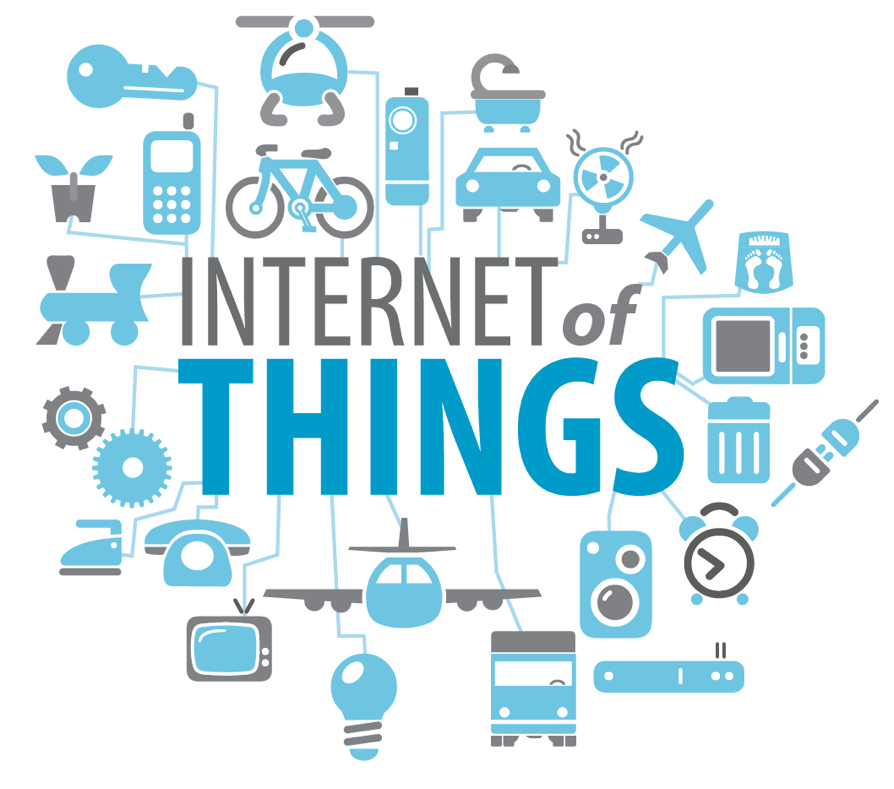
\includegraphics[width=\textwidth]{iot_wstep}
\caption{IoT, źródło: http://knowledge-cess.com/category/technical/iot-internet-of-things/, data pobrania: 20.05.2016}
\label{fig:iot}
\end{figure}

Internet jest znany na całym świecie, przeciętnemu użytkownikowi
kojarzy się on z siecią komputerów, które są ze sobą połączone. Dziś internet oznacza dużo więcej niż tylko komputery, przy których siedzą ludzie. Coraz częściej to również urządzenia i maszyny, z których każdy na co dzień korzysta. Takie połączenia miliardów różnych czujników, komputerów i urządzeń uruchamiających, są dużą zmianą w życiu nas wszystkich, dlatego też często mówi się o tym jako o kolejnej rewolucji internetowej.

Termin \emph{„Internet rzeczy”} z ang. \emph{„Internet of Things”}, w skrócie \emph{IoT}, to koncepcja stworzona prze \emph{Kevina Ashtona} podczas prezentacji przygotowanej dla \emph{Procter \& Gamble} w 1999 roku \cite{KA:2009:iot}. Można ja tłumaczyć na wiele różnych sposobów, natomiast najlepiej określa się ją jako ekosystem, w którym przedmioty, dzięki wyposażeniu w sensory, komunikują się z komputerami. Dla wielu ludzi to nadal coś niewyobrażalnego, ale niedługo w jedną sieć będzie połączone ze sobą praktycznie wszystko. Wiele nowych możliwości staje otworem dla ludzi, którzy zajmują się marketingiem i komunikacją, lecz nie tylko. 

Tematem naszej pracy jest przybliżenie ideologii \emph{Inteligentnego Domu} z wykorzystaniem \emph{Internet of Things}.Cel jaki obraliśmy to przybliżenie w/w tematyki i obalenie mitu, że owe rozwiązania muszą być kosztowne i skomplikowane do zaimplementowania, w oparciu o Nasze własne doświadczenia oraz trzy projekty, które zostały opisane w owej pracy. Inteligentny Dom to określenie, które mówi o bardzo zaawansowanym technicznie budynku. Nie zawsze jest to budynek mieszkalny, mogą to być także  biura, firmy czy hale produkcyjne. 
Inteligentny budynek charakteryzuje się posiadaniem dużej ilości detektorów i czujników, zamieszczonych w ścianach, podłodze czy przy suficie. Wszystkie instalacje połączone ze sobą, tworzą jeden zintegrowany system zarządzania budynku. Systemy te pozwalają na to, aby budynek mógł reagować na zmiany środowiska. Wszystkie te działania maksymalizują komfort użytkowania, funkcjonalność oraz bezpieczeństwo. Dzięki nim możemy także zaoszczędzić energię czy wodę, zmniejszają więc koszty eksploatacji, a także pozwalają na zmniejszenie emisji zanieczyszczeń do środowiska. 
Podstawę do napisania pracy stanowił projekt, na który wpadł mój kolega parę lat temu (\emph{www.windfreaks.pl}), który miał wspierać naszą pasję jaką jest kiteboarding poprzez budowę kilku stacji pogodowych oraz kamer HD rozciągniętych wzdłuż wybrzeża zatoki Gdańskiej oraz półwyspu Helskiego miało to na celu dostarczanie rzetelnych danych pogodowych.  Również jednym z głównych źródeł była książka Michaela Millera pt. „The Internet of Things: How Smart TVs, Smart Cars, Smart Homes, and Smart Cities Are Changing the World” \cite{MM:2015:TIOT}, z której dowiedzieliśmy się w jaki sposób połączone urządzenia mogą poprawić nasze życie prywatne, a także prowadzony biznes, co się dzieje z danymi gromadzonymi w sieci, czy można dzięki niemu zdrowiej żyć czy oszczędzać energię, oraz jakie zagrożenia niesie za sobą IoT. Ważną rolą w przygotowaniu pracy był raport „Internet Rzeczy w Polsce” \cite{RP:2015:IOTPL} oraz książka „Internet rzeczy, Bezpieczeństwo w Smart City”, wydawnictwa C.H. Beck \cite{beck}. 
Praca składa się ze wstępu, trzech rozdziałów merytorycznych oraz zakończenia. Wstęp zawiera ogólny opis problematyki pracy i celów w niej postawionych. Pierwszy rozdział to bardziej szczegółowy opis terminu \emph{„Internet of Things”}, warunki jego istnienia oraz jego korzyści i wyzwania prywatności w Internecie Rzeczy. Drugi rozdział to wgłębienie się w temat warunków i idei rozwoju \emph{IoT} oraz zagrożeń zeń płynących.  W trzecim rozdziale przedstawione zostały szerzej rozwiązania praktyczne w oparciu o rozwiązania dostępne na rynku oraz trzy projekty naszego autorstwa podzielone na projekty:
\begin{itemize}
\item inteligentnego nawadniania roślin
\item własnego systemu monitoringu
\item inteligentnego systemu oświetleniowego
\end{itemize}

\chapter{Internet rzeczy}


\section{Informacje ogólne o Internetu rzeczy}

Żyjąc w XXI wieku jesteśmy świadkami wielu cyfrowych rewolucji. W 1990 John Romney podłączył toster do sieci internet, który to mógł włączać i wyłączać zdalnie \cite{toster}.Było to pierwsze na świecie urządzenie podłączone do internetu, które zapoczątkowało rewolucje znaną nam jako \emph{Internet Rzeczy}. Otwiera przed nami wiele nowych możliwości komunikacji z konsumentem. Są one szybsze, łatwiejsze i jeszcze bardziej efektywne niż były dotychczas. 
\begin{figure}[h]
\centering
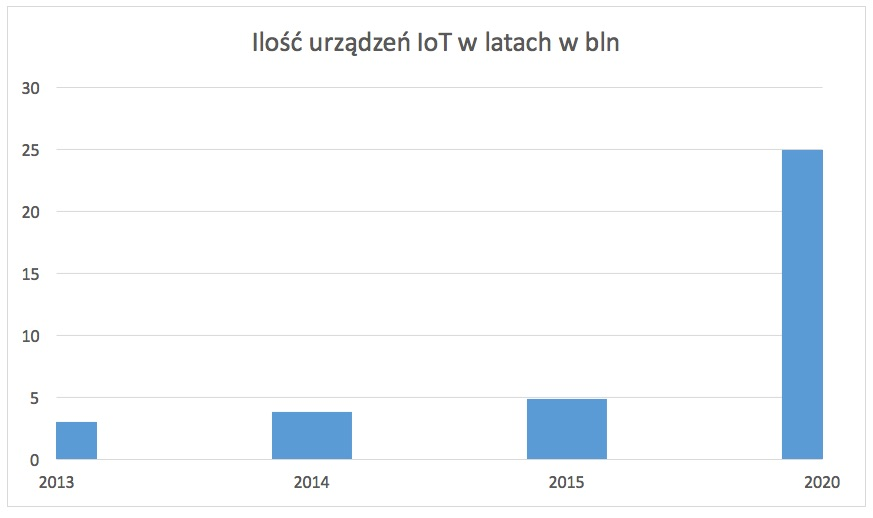
\includegraphics[width=\textwidth]{w}
\caption{Ilość urządzeń IoT , źródło: Gartner, listopad 2014r.}
\label{fig:ilosciot}
\end{figure}
 Pewna część społeczeństwa widzi w \emph{IoT} szanse, inni boją się, że postępująca cyfryzacja za bardzo rozpowszechnia się w naszym życiu. Mimo wszystko, liczba urządzeń podłączonych do Internetu wzrasta w bardzo szybkim tempie i do 2020 roku ma osiągnąć ponad 25 mld urządzeń na całym świecie rys. \ref{fig:ilosciot}.

Internet rzeczy dotyczy przedmiotów, które gromadzą i przetwarzają dane, pośrednio bądź bezpośrednio, dzięki sieci komputerowej. Możemy do nich zaliczyć smartfony i laptopy, a także samochody, sprzęty, biura, fabryki, a nawet całe miasta \cite{miasta}, gospodarkę wodną czy systemy obronne. IoT wpływa między innymi na projektowanie i serwis, a także na zarządzanie zasobami ludzkimi, dzięki czemu stwarza ogromne szanse na „lepsze jutro” w dziedzinie biznesu. 

\section{Warunki istnienia IoT}

Jak już wcześniej wspomniano, IoT może być rozumiany jako ekosystem, w którym komunikacja występuje z udziałem człowieka, lub bez niego. Aby móc wymienić informacje między dwoma przedmiotami, należy spełnić określone warunki.
\begin{figure}[h]
\centering
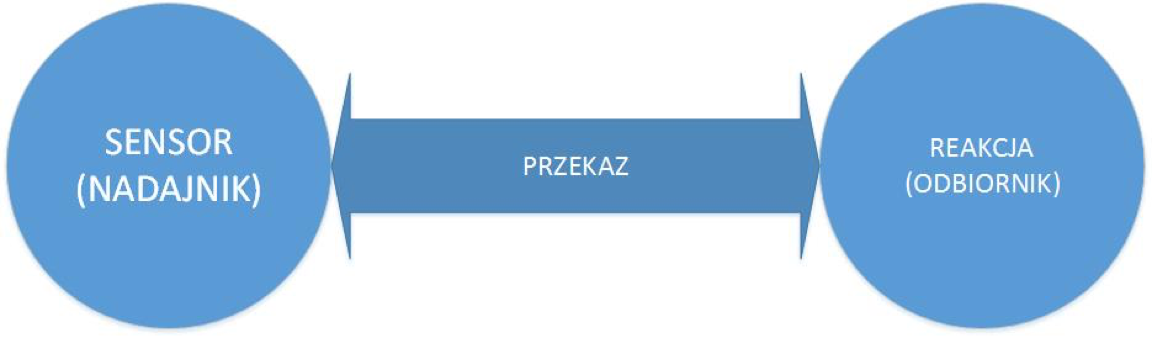
\includegraphics[width=12cm]{o}
\caption{Opracowanie własne}
\label{fig:opracowanie}
\end{figure} 
Pierwszą ważną rzeczą jest fakt, iż przedmiot, który ma wysyłać informacje, musi być wyposażony w sensor. Dzięki niemu jest w stanie zebrać potrzebne dane z otoczenia, aby móc je przekazać odbiorcy rys \ref{fig:opracowanie}. Jako nadajniki mogą posłużyć smartfony, czujniki wilgotności, temperatury czy ruchu. Różnica między tymi czujnikami a smartfonem jest taka, iż ze smartfona dane są wysyłane dzięki akcji, którą wyzwala człowiek. Przykładami ostatnio bardzo modnymi mogą być opaski mierzące tętno, czy liczące ilość wykonanych kroków w ciągu dnia, a także mniej popularne jeszcze w Polsce prześcieradła z czujnikami ruchu. 
Kolejnym warunkiem, jaki musi być spełniony jest to, że przedmiot, który będzie odbierał sygnał przesłany przez nadawcę, musi być w stanie go odebrać, przetworzyć i wywołać odpowiednią relacje. Przy takich odbiornikach jak komputer czy telefon, informacja przesłana wyświetli się na ekranie. Mogą to być także urządzenia, które wykonają określoną czynność, a nie wyświetlą samej informacji. Przykładem może być układ nawadniania, który automatycznie włączy wodę, bądź kontroler oświetlenia, który o zmierzchu włączy światło, czy też rolety, które zasłonią się lub odsłonią o odpowiedniej porze. Bardziej abstrakcyjnymi przykładami mogą być książki, które wyświetlą datę zwrotu do biblioteki, czy też lodówki pokazujące braki w zaopatrzeniu domowej spiżarni~\cite{Designing}.  
Trzecia rzeczą potrzebną do stworzenia takiej relacji jest środek komunikacji, czyli to w jaki sposób dane zostaną przesłane od nadawcy do odbiorcy. Najbardziej popularne w dzisiejszych czasach to WiFi czy Bluetooth, a mniej znane dla przeciętnego użytkownika internetu NFC czy Z-WAVE, które wykorzystywane są w systemach budynków. 
Relację opisanych wyżej trzech rzeczy obrazuje rysunek 3.

\section{Korzyści wynikające z wykorzystania internetu rzeczy}
Tak szybki rozwój technologii i łączności otwiera drogę na coraz bardziej nowatorskie i zaawansowane rozwiązania ułatwiające ludziom życie. Największy potencjał w tej dziedzinie ma inteligentny dom. Dom jest miejscem, gdzie czujemy się bezpiecznie i zawsze możemy tu wrócić. Nic więc dziwnego, że stale chcemy ułatwiać sobie życie dostosowując otaczającą nas elektronikę do naszych potrzeb.
O ile do niedawna możliwość posiadania inteligentnego domu zarezerwowana była tylko dla osób, które same były sobie taki dom skonstruować to teraz jest co raz więcej firm które zrobią to za nas. Idea tzw. „smart home” jest najszybciej rozwijającą się ideą w dziedzinie Internetu Rzeczy. Niemiecki koncern zajmujący się badaniem opinii publicznej GfK przeprowadził w 2015 roku analizę rynku inteligentnych domów. Gwałtowny rozój technologii, co raz więcej przedsiębiorstw interesujących się tematem oraz prognozy firmy GSMA, która w 2011 roku oszacowała rynek inteligentnych domów na 40 miliardów dolarów, przyczyniły się do powstania raportu GfK. Badaniu poddanych zostało ponad 7.000 respondentów z 7 krajów – USA, Wielkiej Brytanii, Niemiec, Japonii, Chin, Brazylii oraz Korei Południowej. Według badań aż 91\% było świadomych co oznacza idea inteligentnego domu, a 68\% badanych posiadała ogólną wiedzę na ten temat. To bardzo dobry wynik jak na ideę, o której do niedawna w ogóle się nie mówiło.
Raport również ukazuje, że 55\% badanych uważa bezpieczeństwo za jeden z ważniejszych aspektów. Mowa oczywiście o monitoringu, alarmach i systemach zapobiegawczych. Jednak ma to swoją ciemną stronę, która zostanie dokładnie opisana w następnym rozdziale.~\cite{Gfk:2015:CMC}
Aby „poczuć ducha” inteligentnego domu wcale nie trzeba wydawać dużych pieniędzy – każdy z minimalną wiedzą informatyczną jest w stanie samemu stworzyć sobie taki dom, na większą lub mniejszą skalę. Wystarczy komputer i dobry pomysł aby przekształcić swoje cztery kąty w coś wyjątkowego.

Głównym kierunkiem rozwoju jest zwiększenie relacji pomiędzy człowiekiem, a przedmiotem, a to wywołuje potrzebę analizy coraz większej ilości danych. 
Jest wiele korzyści wynikających z korzystania z rozwiązań IoT. Zalicza się do nich oszczędność zużycia energi, lepszą kondycję fizyczną oraz zdrowie własne i bliskich. Ważną rzeczą jest też większe poczucie kontroli nad urządzeniami i sprzętami. Następną korzyścią jest zwiększenie produktywności i bezpieczeństwa kadry pracowniczej oraz poprawa relacji z klientem, dzięki zwiększonej komunikacji.

\chapter{Kierunki rozwoju Internetu Rzeczy}

\section{Warunki rozwoju IoT}

Są trzy poziomy dojrzałości, dzięki którym możemy zauważyć bezpośrednie korzyści biznesowe.1
Pierwszy poziom „Data to Discovery”, mówi o bazie nowych danych i ich wykorzystaniu, w celu  zdobycia informacji o rzeczach, o których nie wiedziano dotychczas. Przykładem może być odnalezienie nowych wzorców choroby dzięki informacji z maszyn medycznych. 
Drugim poziomem dojrzałości jest „Data to Decisions”, w którym mowa o tym, że na bazie odpowiednich danych można podjąć autonomicznie akcje, na przykład awaryjne wyłączenie urządzenia w momencie awarii. 
Ostatnim poziomem jest „Data To Dollors-Dividents”, gdzie widać korzyść finansową dla firmy bądź szanse jej rozwoju, gdy połączy się dwa wcześniejsze poziomy ze sobą oraz wprowadzi usługi i produkty innowacyjne. 
Media społecznościowe wpłynęły znacząco na to jak zaczęto organizować swoje życie, oraz zmieniły one modele biznesowe. Tak samo Internet rzeczy znalazł już swoje miejsce. Można powiedzieć, że jest on etapem rewolucji informacyjnej. Dostarczamy techniki i narzędzia, dzięki którym możemy budować wiedzę. Na dużych i szybkich strumieniach danych, nowoczesne urządzenia są w stanie podejmować odpowiednie decyzje. Sukcesu można się spodziewać, jeżeli wprowadzi się innowacyjne zastosowania w nowej przestrzeni. 
Na rozwój IoT miało wpływ wiele rzeczy. Jedną z nich i najważniejszą jest miniaturyzacja. Dzięki niej możemy wszędzie umieścić mikroelementy (czujniki, komputery). Ważną rolę odegrała też technologia mobilna, która ciągle się rozwija. Ostatnią znaczącą rolą, bez której IoT by nie istniało jest bezprzewodowa sieć internetowa. 
Niestety istnieje kilka barier rozwojowych dla tematu IoT. Pierwsza to problem zasilania. Każde urządzenie, nawet to, w którym jest bardzo mocna bateria, wymagać będzie w końcu podłączenia do prądu. Kolejną barierą jest ilość tylko 4 mld urządzeń, które mogą posiadać adres IPv4. Aby rozwiązać ten problem należy używać adresu IPv6, który ma dużo więcej kombinacji ze względu na to, że jest dłuższy od wersji czwartej. Ostatnią barierą, która zostanie przytoczona jest bezpieczeństwo danych i prywatność. Przekonanie ludzi, że informacje są chronione jest bardzo trudne, ale możliwe. Przykładem tego zjawiska są banki. Jeżeli dane między urządzeniami będą tak samo zabezpieczone jak środki na internetowym rachunku bankowym to Internet of Things stanie się rzeczywisty~\cite{KeyApplications}.

\section{Idea rozwoju Internetu Rzeczy}
Dla przeciętnego człowieka internet to połączone w sieć komputery, które wymieniają się danymi. Internet jest dla niego miejscem czerpania wiedzy i rozrywki, komunikowania się ze znajomymi i wrażania swoich opinii. Jest to dla niego otwarty, częściowo anonimowy wirtualny świat, zupełnie inny od tego w którym żyje na co dzień. Początki internetu były bardzo skromne ale teraz jest to ogromna sieć łącząca ze sobą już nie tylko komputery, ale też telefony czy nawet urządzenia gospodarstwa domowego. Internet rozrasta się w tempie wykładniczym – jego rozwój niesie za sobą ogromne korzyści, ale również poważne zagrożenia.~\cite{Nsr:2015:CMC}
\begin{figure}[h]
\centering
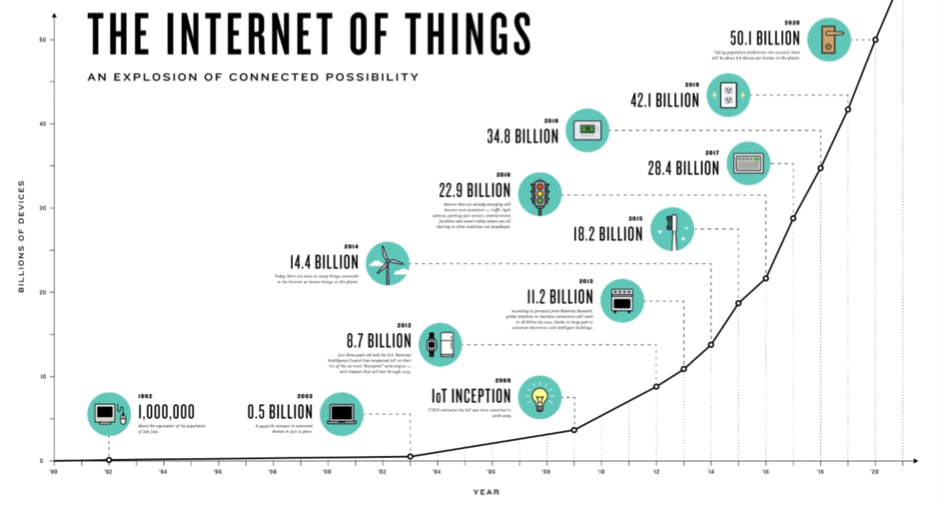
\includegraphics[width=12cm]{m_exp}
\caption{IoT: An explosion of connected possibility. Źródło: http://www.nsr.com/news-resources/the-bottom-line/internet-of-things-prime-time-for-satellite/}
\label{fig:exp}
\end{figure} 
Największym motorem napędowym ekspansji Internetu Rzeczy jest chęć ludzi do ułatwiania sobie życia. Najlepszym tego przykładem jest koncepcja tzw. „Inteligentnego Domu”. Już w tym momencie możemy ustawić pralkę, aby rozpoczęła swoją pracę z opóźnieniem dzięki czemu możemy wrócić do domu akurat gdy pranie się skończy. Możemy zainstalować przełączniki światła sterowane dźwiękiem, dzięki czemu możemy zgasić lub zapalić światło nie wstając z łóżka. Mamy czasowe przełączniki, które symulują obecność domowników podczas ich nieobecności, żelazka, które same się wyłączą po pewnym okresie nieaktywności i tak dalej. Przykładów jest dużo więcej, a codziennie dochodzą nowe urządzenia, które w mniejszym lub większym stopniu ułatwiają nam życie w domu. Jeśli połączymy te wszystkie urządzenia w jedną sieć zarządzaną centralnie możemy mówić o inteligentnym domu. Jest on inteligentny na swój sposób – jest zaprogramowany aby zachowywać się w określony sposób lecz nie jest do końca autonomiczny. Co raz bardziej rozpędzający się postęp technologiczny w połączeniu z nieograniczoną ludzką wyobraźnią tworzy mieszankę wybuchową co wcale nie oznacza najgorszego. Wszak dynamit jest teraz kojarzony z bandytami napadającymi na banki, został wynaleziony w celu ułatwienia wydobywania naturalnych zasobów Ziemi~\cite{Rethinking}.

Internet Rzeczy rozwija się w wielu kierunkach, nawet w dziedzinach które w ogóle nie kojarzą się z elektroniką. Doskonałym przykładem są tzw. „wearables”, czyli przedmioty osobiste które użytkownik nosi na sobie. Są to na przykład smart watch'e, które mają wbudowane moduły łączności bezprzewodowej.  Takie urządzenia mogą mieć dodatkowo wbudowane moduły GPS, co w teorii może znacząco ułatwić wezwanie pomocy w odpowiednie miejsce. Jednak taki zegarek może też przysporzyć wielu kłopotów – gdy osoba trzecia uzyska dostęp do danych lokalizacyjnych  może z łatwością śledzić użytkownika i wykorzystać tę wiedzę do złych celów. Jeśli włamywacz ma absolutną pewność, że dana osoba znajduje się setki kilometrów od domu to bez większego ryzyka nakrycia może ten dom okraść.

Na szczęście rynek wearables jeszcze raczkuje, a najwięcej urządzeń mogących tworzyć Internet of Things powstaje w dziale RTV/AGD. Urządzenia domowe już dawno przyćmiły swoich protoplastów swoją mocą obliczeniową i możliwościami. Współczesne telewizory nie tylko są w stanie wyświetlać obraz nadawany z zewnętrznego urządzenia, ale same potrafią rozkodować sygnał z anteny. Mają własne systemy operacyjne, które implementują możliwości będące do niedawna ekskluzywną domeną komputerów osobistych. Posiadają przeglądarki internetowe, komunikatory a nawet gry. Niektóre mają wbudowane kamerki internetowe, a większość z nich obsługuje peryferyjne urządzenia rejestrujące. Tutaj znowu pojawia się problem, ponieważ owszem te urządzenia wykorzystywane są do prowadzenia wideo-rozmów ale gdy dostęp do nich uzyska niepowołana osoba stwarza to realne zagrożenie dla domowników, nie mówiąc już o utracie jakiejkolwiek prywatności.

Udział sprzętu RTV/AGD w ekosystemie IoT przekracza 30\%~\cite{IotWPolsce:2015:CMC}. Nic w tym dziwnego, skoro cała idea Internetu Rzeczy zrodziła się właśnie w urządzeniach tego typu. Są to na razie tradycyjne sprzęty użytku domowego, czyli np. skanery, telewizory, urządzenia audio. Nowości na rynku sprzętu elektronicznego, takie jak smart lodówki, stanowią znikomy ułamek całego udziału sprzętu RTV/AGD w urządzeniach uważanych jako mogące być częścią IoT.

\section{Wykorzystanie IoT w zyciu codziennym - wearables, RTV/AGD}

Internet Rzeczy rozwija się w wielu kierunkach, nawet w dziedzinach które w ogóle nie kojarzą się z elektroniką. Doskonałym przykładem są tzw. „wearables”, czyli przedmioty osobiste które użytkownik nosi na sobie. Są to na przykład smart watch'e, które mają wbudowane moduły łączności bezprzewodowej. Takie urządzenia mogą mieć dodatkowo wbudowane moduły GPS, co w teorii może znacząco ułatwić wezwanie pomocy w odpowiednie miejsce. Jednak taki zegarek może też przysporzyć wielu kłopotów – gdy osoba trzecia uzyska dostęp do danych lokalizacyjnych może z łatwością śledzić użytkownika i wykorzystać tę wiedzę do nieodpowiednich celów. Jeśli włamywacz ma absolutną pewność, że dana osoba znajduje się setki kilometrów od domu to bez większego ryzyka może ten dom okraść.
Rynek wearables jeszcze raczkuje, a najwięcej urządzeń mogących tworzyć Internet of Things powstaje w dziale RTV/AGD. Urządzenia domowe już dawno przyćmiły swoich protoplastów swą mocą obliczeniową i możliwościami. Współczesne telewizory nie tylko są w stanie wyświetlać obraz nadawany z zewnętrznego urządzenia, ale same potrafią rozkodować sygnał z anteny. Mają własne systemy operacyjne, które implementują możliwości będące do niedawna ekskluzywną domeną komputerów osobistych. Posiadają przeglądarki internetowe, komunikatory a nawet gry. Niektóre mają wbudowane kamerki internetowe, a większość z nich obsługuje peryferyjne urządzenia rejestrujące. Tutaj znowu pojawia się problem, ponieważ owszem te urządzenia wykorzystywane są do prowadzenia wideo-rozmów, ale gdy dostęp do nich uzyska niepowołana osoba stwarza to realne zagrożenie dla domowników, nie mówiąc już o utracie jakiejkolwiek prywatności.
Udział sprzętu RTV/AGD w ekosystemie IoT przekracza 30. Nic w tym dziwnego, skoro cała idea Internetu Rzeczy zrodziła się właśnie w urządzeniach tego typu. Są to na razie tradycyjne sprzęty użytku domowego, czyli np. skanery, telewizory, urządzenia audio. Nowości na rynku sprzętu elektronicznego, takie jak smart lodówki, stanowią znikomy ułamek całego udziału sprzętu RTV/AGD w urządzeniach mogących być częścią IoT.

\section{Inteligetny Dom}

Szybki rozwój technologii i łączności otwiera drogę na coraz bardziej nowatorskie i zaawansowane rozwiązania ułatwiające ludziom życie. Największy potencjał w tej dziedzinie ma inteligentny dom. Dom jest miejscem, w którym czujemy się bezpiecznie i zawsze możemy do niego wrócić. Nic więc dziwnego, że stale chcemy ułatwiać sobie życie dostosowując otaczającą nas elektronikę do naszych potrzeb.
O ile do niedawna możliwość posiadania inteligentnego domu zarezerwowana była tylko dla osób, które same były w stanie sobie taki dom skonstruować to teraz jest coraz więcej firm które zrobią to za nas. Idea tzw. „smart home” jest najszybciej rozwijającą się ideą w dziedzinie Internetu Rzeczy. Niemiecki koncern zajmujący się badaniem opinii publicznej „GfK” przeprowadził w 2015 roku analizę rynku inteligentnych domów. Gwałtowny rozwój technologii, coraz więcej przedsiębiorstw interesujących się tematem oraz prognozy firmy GSMA, która w 2011 roku oszacowała rynek inteligentnych domów na 40 miliardów dolarów~\cite{Gsma:2011:CMC}, przyczyniły się do powstania raportu „GfK”. Badaniu poddanych zostało ponad 7.000 respondentów z 7 krajów – USA, Wielkiej Brytanii, Niemiec, Japonii, Chin, Brazylii oraz Korei Południowej. Według badań aż 91\% było świadomych, co oznacza idea inteligentnego domu, a 68\% badanych posiadało ogólną wiedzę na ten temat. To bardzo dobry wynik jak na ideę, o której do niedawna w ogóle się nie mówiło.
\begin{figure}[h]
\centering
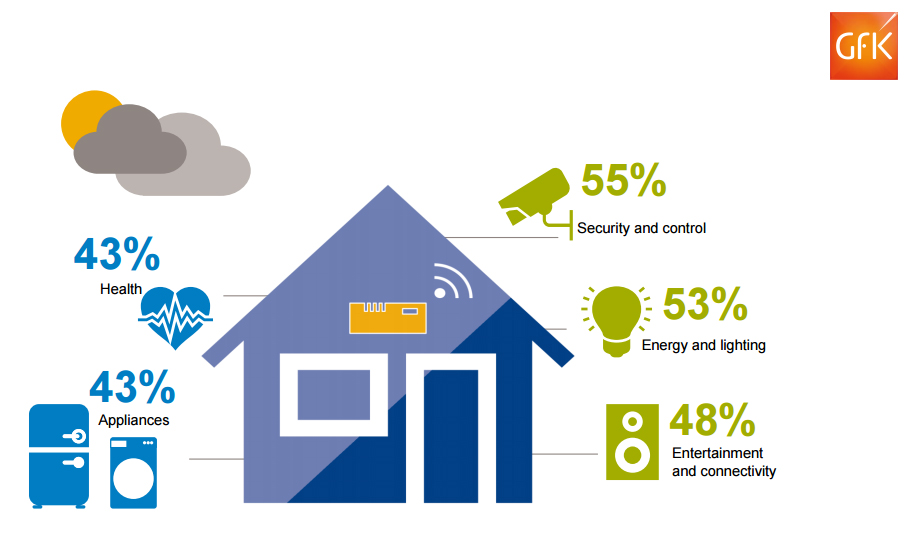
\includegraphics[width=12cm]{m_percent}
\caption{GfK report on Internet of Things. Źródło: https://www.gfk.com/fileadmin/user_upload/dyna_content/Global/documents/Reports/GfK-smart-home-teaserdeck-global.pdf}
\label{fig:gfk}
\end{figure} 

\section{Zagrożenia płynące z rozwoju IoT}
Urządzenia, z których korzystamy na co dzień są co raz bardziej złożone. Ma to na celu oczywiście ułatwienie życia i umożliwienie dokonywania rzeczy które wcześniej istniały tylko w sferze fantastyki. 

Najbardziej niebezpieczne wydają się wspomniane wcześniej wearables. Z definicji nosimy je zawsze przy sobie i to one stanowią największe niebezpieczeństwo dla użytkownika oraz są najbardziej podatne na utratę prywatności. Przykładem nasuwającym się od razu na myśl jest Google Glass. Dodatkowo zaciera się granica między rodzajami Rzeczy Internetu – Google Glass może być używane do kontrolowania domu, i osoby trzecie, które uzyskają dostęp do urządzenia, będą w stanie kontrolować cały dom i potencjalnie  szpiegować domowników.
To urządzenie może wkrótce zrewolucjonizować rynek urządzeń mobilnych. Jednak niesie to za sobą poważne zagrożenia. Google Glass do komunikacji z siecią może używać albo połączenia Bluetooth, albo Wi-Fi. W przypadku tego pierwszego potrzebne jest dodatkowe urządzenie służące jako punkt dostępowy dla okularów od internetowego giganta. Druga opcja jest bardziej przystępna, gdyż nie wymaga od użytkownika posiadania przy sobie innego urządzenia mobilnego z dostępem do sieci. Jednak jak zauważa Roberto Martinez, badacz z Kaspersky Lab, który przyjrzał się sprawie bezpieczeństwa Google Glass, komunikacja Wi-Fi naraża urządzenie na ataki hakerów. Martinez i Juan Andres Guerrero – kolega z zespołu badawczego – przeprowadzili eksperyment w monitorowanej sieci. Odkryli, że tylko część danych wymienianych między urządzeniem a punktem dostępowym była szyfrowana. Badaczom udało się ustalić, że „ofiara” szukała połączeń lotniczych oraz miejscowości turystycznych. Potencjalny haker prawdopodobnie mógłby wyciągnąć jeszcze więcej informacji, gdyby tylko poświęcił na to więcej czasu~\cite{Abusing}.

“We admit that it is not a very damaging vulnerability, but even so, profiling via meta data from Web traffic exchange could become the first step of a more complex attack against the device’s owner.” - Roberto Martinez
Kolejnym całkiem nowym na rynku urządzeniem które potencjalnie może przysporzyć właścicielowi kłopotów jest Galaxy Gear 2 od Samsunga. Jest to tzw. smartwatch – zegarek, który potrafi dużo więcej niż tylko wskazać godzinę. Eksperci z Kaspersky Lab również przyjrzeli się temu akcesorium i zarówno jak i w przypadku Google Glass jak i tutaj znaleźli potencjalne zagrożenia dla użytkownika. Pierwszą rzeczą, na jaką zwrócili uwagę badacze był aparat. Samsung dobrze zdawał sobie sprawę, że umieszczanie miniaturowego aparatu w bardzo małym, niepozornym urządzeniu może narobić komuś szkody. Dlatego zegarek wydaje głośny dźwięk za każdym razem gdy robione jest zdjęcie i nie umożliwia wyłączenia tej opcji w żaden sposób. Ma to na celu ostrzeżenie ludzi dookoła, że potencjalnie zostało zrobione im zdjęcie. Jednak pracownicy Kaspersky Lab znaleźli obejście tego zabezpieczenia. Wystarczy tylko uzyskać dostęp administratora (tzw. root) co jest trywialnie proste mając fizyczny dostęp do urządzenia i użyć ogólnodostępnego narządzia ODIN od Samsunga. Wyłączając dźwięk migawki nie tylko umożliwiamy właścicielowi zegarka robienie tajnych zdjęć innym osobom, ale też umożliwiamy hakerowi robienie zdjęć właścicielowi, tego co robi i gdzie jest – bez jego wiedzy.

Innym problemem Galaxy Gear 2 jest sposób, w jaki instalowane są aplikacje. Używane jest do tego oficjalne oprogramowanie od Samsunga – Gear Manager – jednak sposób w jaki aplikacja wgrywa inne programy do akcesorium pozostawia duży potencjał hakerski. Na zegarku nie wyświetla się żadna informacja o instalowanym oprogramowaniu, co umożliwia instalowanie złośliwych aplikacji bez wiedzy posiadacza. W połączeniu z wiedzą jak ukrywać zainstalowane już aplikacje na systemie Android, na którym Galaxy Gear 2 operuje, daje to nieograniczone możliwości dla hakerów.

Na szczęście są to urządzenia dosyć młode na rynku sprzętu elektronicznego i zagrożenia związane z włamywaniem się na nie nie są aż tak powszechne. Jak zaznacza Juan Andres Guerrero na chwilę obecną nie ma żadnych dowodów sugerujących, że wearables są celem hakerów jednak to może się zmienić w przyszłości, gdy staną się bardziej powszechne.

Aby „poczuć ducha” inteligentnego domu wcale nie trzeba wydawać dużych pieniędzy – każdy z minimalną wiedzą informatyczną jest w stanie samemu stworzyć sobie taki dom, na większą lub mniejszą skalę. Wystarczy komputer i dobry pomysł, aby przekształcić swoje cztery kąty w coś wyjątkowego.
Urządzenia, z których korzystamy na co dzień są coraz bardziej złożone. Ma to na celu oczywiście ułatwienie życia i umożliwienie dokonywania rzeczy, które wcześniej istniały tylko w sferze fantastyki.
Najbardziej niebezpieczne wydają się wspomniane wcześniej wearables. Z definicji nosimy je zawsze przy sobie i to one stanowią największe niebezpieczeństwo dla użytkownika oraz stanowią największe zagrożenie utraty prywatności. Przykładem nasuwającym się od razu na myśl jest Google Glass. Dodatkowo zaciera się granica między rodzajami Rzeczy Internetu – Google Glass może być używane do kontrolowania domu, i osoby trzecie, które uzyskają dostęp do urządzenia, będą w stanie kontrolować cały dom i potencjalnie  szpiegować domowników.~\cite{Kaspersky:2014:CMC}

Ten wynalazek może wkrótce zrewolucjonizować rynek urządzeń mobilnych. Jednak niesie to za sobą poważne zagrożenia. Google Glass do komunikacji z siecią może używać albo połączenia Bluetooth, albo Wi-Fi. W przypadku tego pierwszego potrzebne jest dodatkowe urządzenie służące jako punkt dostępowy dla okularów od internetowego giganta. Druga opcja jest bardziej przystępna, gdyż nie wymaga od użytkownika posiadania przy sobie innego urządzenia mobilnego z dostępem do sieci. Jednak jak zauważa Roberto Martinez1 badacz z Kaspersky Lab, który przyjrzał się sprawie bezpieczeństwa Google Glass, komunikacja Wi-Fi naraża urządzenie na ataki hakerów. Martinez i Juan Andres Guerrero – kolega z zespołu badawczego – przeprowadzili eksperyment w monitorowanej sieci. Odkryli przypis, że tylko część danych wymienianych między urządzeniem a punktem dostępowym była szyfrowana. Badaczom udało się ustalić, że „ofiara” szukała połączeń lotniczych oraz miejscowości turystycznych. Potencjalny haker prawdopodobnie mógłby wyciągnąć jeszcze więcej informacji, gdyby tylko poświęcił na to więcej czasu.
“We admit that it is not a very damaging vulnerability, but even so, profiling via meta data from Web traffic exchange could become the first step of a more complex attack against the device’s owner,” - Roberto Martinez2
Kolejnym całkiem nowym na rynku urządzeniem które potencjalnie może przysporzyć właścicielowi kłopotów jest Galaxy Gear 2 od Samsunga. Jest to tzw. smartwatch – zegarek, który potrafi dużo więcej niż tylko wskazać godzinę. Eksperci z Kaspersky Lab przyjrzeli się również temu akcesorium i zarówno w przypadku Google Glass jak i tutaj znaleźli potencjalne zagrożenia dla użytkownika. Pierwszą rzeczą, na jaką zwrócili uwagę badacze był aparat. Samsung dobrze zdawał sobie sprawę, że umieszczanie miniaturowego aparatu w bardzo małym, niepozornym urządzeniu może narobić komuś szkody. Dlatego zegarek wydaje głośny dźwięk za każdym razem gdy robione jest zdjęcie i nie umożliwia wyłączenia tej opcji w żaden sposób. Ma to na celu ostrzeżenie ludzi dookoła, że potencjalnie zostało zrobione im zdjęcie. Jednak pracownicy Kaspersky Lab znaleźli obejście tego zabezpieczenia. Wystarczy tylko uzyskać dostęp administratora (tzw. root), co jest trywialnie proste mając fizyczny dostęp do urządzenia, i użyć ogólnodostępnego narządzia ODIN od Samsunga. Wyłączając dźwięk migawki nie tylko umożliwiamy właścicielowi zegarka robienie tajnych zdjęć innym osobom, ale też umożliwiamy hakerowi robienie zdjęć właścicielowi, tego co robi i gdzie jest – bez jego wiedzy.
Innym problemem Galaxy Gear 2 jest sposób, w jaki instalowane są aplikacje. Używane jest do tego oficjalne oprogramowanie od Samsunga – Gear Manager – jednak sposób w jaki aplikacja wgrywa inne programy do akcesorium pozostawia duży potencjał hakerski. Na zegarku nie wyświetla się żadna informacja o oprogramowaniu, co umożliwia instalacje złośliwych aplikacji bez wiedzy posiadacza. W połączeniu z wiedzą jak, ukrywać zainstalowane już aplikacje na systemie Android, na którym Galaxy Gear 2 operuje, daje to nieograniczone możliwości dla hakerów.
Na szczęście są to urządzenia jest młode na rynku sprzętu elektronicznego i zagrożenia związane z włamywaniem się na nie nie są aż tak powszechne. Jak zaznacza Juan Andres Guerrero3 na chwilę obecną nie ma żadnych dowodów sugerujących, że wearables są celem hakerów, jednak to może się zmienić w przyszłości, gdy staną się bardziej powszechne.
“At this time there is no evidence to suggest that wearables are currently being targeted by professional APT actors. However there is a twofold appeal presented by wearables that make them a likely future target if they are widely adopted by consumers.  In future the data collected by wearable devices is going to attract new players to the cyber-espionage scene.” -  Juan Andres Guerrero4
Niebezpieczeństwa niesione przez IoT można rozpatrywać na dwa sposoby: niebezpieczeństwa związane z informatyzacją świata konsumenckiego oraz optymalizacją sektora przemysłowego~\cite{Ks:2014:CMC}. W czasach rozpędzającego się rozwoju Internetu Rzeczy, ludzie skazani są na informatyzację większości dziedzin życia. Inteligentny sprzęt gospodarstwa domowego, elektroniczne zamki do drzwi lub okien, liczniki energii, itd. Wszystkie te sprzęty niosą za sobą spore niebezpieczeństwo, a ich przeciętni użytkownicy nie zdają sobie sprawy z powagi zagrożenia. Bo przecież dlaczego ktoś miałby się bać swojej lodówki? Otóż wszystko wskazuje na to, że niedługo lodówki będą w stanie gromadzić informacje na temat ich zawartości. Wiedza ta w niepowołanych rękach może zaszkodzić użytkownikowi. Na pewno nie w bezpośredni sposób, bo dieta ofiary nie może być wykorzystana np. do kradzieży pieniędzy z konta bankowego. Umożliwi tzw. profilowanie ofiary. Tak niepozorna wiedza jak to co kto je na śniadanie, w połączeniu z innymi, teoretycznie bezpiecznymi informacjami jak np. godzina o której ofiara rano wstaje (wykradziona ze smartwatch'a) oraz np. ile ciepłej wody zużywa ofiara (wiedza wykradziona z elektronicznych liczników wody). Tak nagromadzona wiedza, pozornie nieprzydatna z punktu widzenia hakera, pozwala na dokładną inwigilację ofiary, poznanie jej nawyków oraz sposobu w jaki żyje stylu życia. Taka wiedza może narobić ofierze wielu problemów gdy znajdzie się w niepowołanych rękach.

\chapter{Doswiadczenia praktyczne}

\section{Wykorzystanie Arduino przy budowaniu własnych projektów}

Przygodę z Internetem rzeczy możemy zacząć od kupienia gotowych rozwiązań. Daje nam to możliwość stworzenia inteligentnego domu całkowicie samodzielnie. Zakup przykładowego zestawu inteligentnych żarówek pozwala nam na sterowania oświetleniem w całym mieszkaniu za pomocą aplikacji na telefon. Jeżeli zaopatrzymy się w odpowiedni model żarówki, możemy również zmieniać kolor oświetlenia oraz jego intensywność. 
Zaopatrywanie się w gotowe przedmioty ma też swoje wady. Jesteśmy ograniczeni przez producenta funkcjonalnością. Programy obsługujące inteligentne rzeczy są pisane pod konkretny ekosystem (Android, iOS, Windows Phone) aplikacja może nie działać na naszym urządzeniu. Narażeni jesteśmy wtedy na dodatkowe koszty - zakup sprzętu, lub musimy szukać innego, często gorszego rozwiązania. Jako osoba studiująca na kierunku Informatyki postanowiłem stworzyć inteligentny przedmiot, który będzie działał tak jak go zaprogramuje. 
Na przeciw moim oczekiwaniom wyszedł Projekt Arduino. Powstał on w 2005 roku we Włoszech. Jest to platforma dla systemów wbudowanych, oparta o 8-bitowe mikrokontrolery Atmel AVR. Płytka posiada ustandaryzowany układ wyjścia-wejścia (ang. input-output circuit, I/O circuit) umożliwia nam  to korzystanie z urządzeń zewnętrznych takich jak: czujniki, sterowników, silniki, wyświetlacze itp. Istnieje kilka wersji płytek Arduino jednak większość z nich nie wymaga żadnego zewnętrznego programatora. Do wgrania oprogramowania wystarczy podłączyć mikrokontroler do komputera. Arduino posiada własne darmowe środowisko - Arduino IDE. Ogromną zaletą platformy jest jej popularność. Dzięki niej w sieci istnieje duża ilość bibliotek do obsługi różnych urządzeń zewnętrznych. Jest także sporo poradników i przykładów zastosowania mikrokontrolera AVR.
Jest to idealne środowisko dla programistów, którzy są pasjonatami elektroniki ale nie lubią konfiguracji programatorów, sprawdzania układów i instalacji sterowników. Do napisania pierwszego programu i uruchomieniu go na Arduino wystarczy nam komputer, przewód miniUSB-USB oraz sama płytka. 

Na początku przygody z płytką Arduino zazwyczaj nie mamy zbyt wiele sprzętu którego moglibyśmy wykorzystać do stworzenia czegoś użytecznego. Dlatego pierwszym programem dzięki którym poznajemy się z samym językiem programowania oraz samym mikrokontrolerem jest miganie wbudowaną diodą.

Inteligentny Dom w praktyce – Stacja Meteorologiczna
Jednym z najprostszych a dającym najwięcej satysfakcji projektów jest stacja meteorologiczna zbudowana przy pomocy Arduino oraz kilku czujników. Poziom zaawansowania układu zależy tutaj od budującego taką stacje. Możemy po prostu mierzyć temperaturę oraz wilgotność powietrza za pomocą cyfrowego czujnika DHT11 lub DHT22. Różnice między czujnikami znajdują się poniżej. 

Jednak taka prosta stacja to nic innego jak domowy termometr. W inteligentnym domu chodzi o coś więcej. Wspomniany projekt możemy rozbudować o kilka dodatkowych sensorów i stworzyć coś na prawdę fajnego. 
Dorzucając takie funkcjonalności jak: wykrywanie burzy, pomiar ciśnienia, sprawdzanie prędkości oraz kierunku wiatru. Jednocześnie wysyłając wszystkie dane do sieci tak, żeby mieć wgląd w historię pogody. Możemy wykorzystać naszą stację jako centrum informacji dla osób zainteresowanych sportami w których wiatr odgrywa kluczową rolę np. windsurfing, kitesurfing. 

Itenligentny Dom w praktyce - Sterowanie oświetleniem
Za pomocą Arduino jesteśmy w stanie sterować oświetleniem w całym mieszkaniu. Wystarczy, że odpowiednio podłączymy moduły z przekaźnikiem do sterownika. Możliwości tego rozwiązania są dużo większe niż wspomniane na początku rozdziału gotowe urządzenia. Tutaj cała konfiguracja i pole manewru leży w naszych rękach. Możemy odwzorować sklepową wersję inteligentnej żarówki i ograniczyć się do centralnego sterowania oświetleniem w domu z poziomu aplikacji na komórce.
Fajnym pomysłem na urozmaicenie takiego projektu jest zaprogramowanie różnych scen. Jednym kliknięciem możemy ustawić oświetlenie tak by sprzyjało czytaniu książki lub oglądaniu filmów.
Kolejnym ciekawym rozwiązaniem jest podpięcie całego systemu oświetlenia do sieci i umożliwienie sterowania przez stronę www. Możemy w ten sposób na przykład sprawdzić czy na pewno zgasiliśmy światło w domu, będąc jednocześnie w zupełnie innym miejscu. Oczywiście trzeba uwzględnić zabezpieczenie takiego projektu tak, żeby osoby niepożądane nie mogły przejąć kontroli nad naszym systemem. Zdalne sterowanie oświetleniem daje nam możliwość symulowania obecności w domu gdy jesteśmy np. na wczasach. Możemy zdalnie włączać i wyłączać światło, ale nic nie stoi na przeszkodzie by ten proces zautomatyzować i ustawić godziny w których nasz dom będzie zapalał i gasił oświetlenie.
W ubiegłym roku powstała strona na której można było sterować oświetleniem świątecznym rozwieszonym na domu. Był jednocześnie podgląd online dzięki któremu na żywo mogliśmy obserwować wszystkie czynności które wykonywaliśmy. 

\section{Projekt inteligentnego nawadniania roślin}

Głównym celem rozdziału poświęconego tworzeniu własnych rozwiązań do inteligentnego domu było stworzenie systemu który pozwoli przy pomocy sensorów wyhodować roślinę. Chcieliśmy też zebrać wszelkie informacje o warunkach w jakich roślina byłaby wyhodowana: temperatura, wilgotność powietrza, wilgotność gleby, poziom natężenia światła. Wszystkie informacje wysyłane są na stronę internetową. Dzięki temu mielibyśmy wgląd do historii danych o warunkach w jakich rosła roślina. 

Pierwszą rzeczą jaką wykonaliśmy to skompletowanie listy rzeczy które będą potrzebne do wykonania tego systemu. Chcieliśmy też osiągnąć cel jak najniższym kosztem. Postanowiliśmy, że zamówimy przedmioty w Chinach, za pośrednictwem portalu www.aliexpress.com. Ceny elementów są dużo niższe niż w Polsce, a jedyna wadą tego rozwiązania był czas realizacji zamówienia który sięgał blisko 60 dni.

Lista zakupów:
\begin{itemize}
\item Płytka Arduino UNO: 2,7
\item Sensor wilgotności gleby: 0,86
\item Sensor temperatury i wilgotności powietrza: 3,01
\item Czujnik natężenia światła: 1,42
\item Moduł Wifi: 2,70
\item Zestaw kabli i rezystorów: 2,00
\item Płytka stykowa dedykowana do Arduino: 1,31
\end{itemize}
Łączna kwota: 14\$
Daje nam to w przeliczeniu: 53,76 zł (przy kursie dolara wynoszącym 3,84 zł)
Gdybyśmy chcieli zrobić takie zakupy w Polsce cena wyniosła by około: 130 zł 

\section{Budowa własnego systemu monitoringu}

Wygodny nadzór nad domem podczas nieobecności do niedawna kojarzył się z czymś ekskluzywnym. Powszechnie monitoring znajdował się jedynie w bogatych domach. Jednak z tak szybkim postępem technologicznym na tego typu luksusy może pozwolić sobie niemalże każdy, praktycznie zerowym kosztem. Większość ludzi posiada jakiś stary, nieużywany telefon komórkowy z aparatem. Można go wykorzystać jako kamerę IP, dostępną w sieci lokalnej domu. Specjalne oprogramowanie będzie przesyłać obraz z dobrze umiejscowionego telefonu do serwera. To może być dowolne urządzenie, jednak na potrzeby naszego eksperymentu będzie nazywany serwerem. W naszym przypadku użyliśmy 2 aparatów i laptopa~\cite{Learning}.
Za strumieniowanie wideo z kamery odpowiedzialny jest program IP Webcam1. Aplikacja jest dostępna za darmo, z możliwością wykupienia wersji pro. W cenie ok. 12 zł znajdują się dodatkowe funkcje:
Integracja z Taskerem,
Konfigurowalny UI,
Bezpośredni skrót na ekranie głównym do uruchomienia aplikacji w, trybie nadawania,
Brak znaku wodnego,
Brak reklam.
To bardzo niewielki koszt w porównaniu z tym, co aplikacja ma do zaoferowania. Autor programu, Pavel Khlebovich, do wersji pro  podchodzi bardziej jak do dobrowolnej dotacji.

IP Webcam posiada ogrom funkcji. Oprócz najważniejszej, czyli wystawiania zwykłego interfejsu kamery IP, sama w sobie posiada funkcję serwera, i to bardzo przemyślanego. Na wstępie zaskakuje ilość sposobów w jaki można odbierać obraz i/lub dźwięk z urządzenia. Można też zapisywać pliki w archiwum, albo skonfigurować Taskera. Wszystko jest zrobione w Bootstrap'ie i działa bardzo dobrze na prawie każdym urządzeniu, dzięki możliwości wyboru sposobu transmisji.
Ma to niestety podstawowy problem. Ciężko mówić o monitoringu, mając obraz z jednej kamery. Wiele kamer oznacza wiele serwerów, każdy nadający obraz tylko ze swojego aparatu. Aby będąc na urlopie podejrzeć obraz z domu, należałoby zalogować się na każdą kamerę z osobna, co w przypadku większej ilości kamer byłoby zupełnie niepraktyczne. Zaprogramowaliśmy serwer w technologii Meteor, który odbiera sygnał z wielu kamer, inaczej, zapisuje migawki do pliku i serwuje je klientowi~\cite{Started}.
Aby to wszystko było możliwe najpierw zainstalowano Meteora. Po początkowych nieudanych próbach uruchomienia frameworka na wirtualnej maszynie VirtualBox + Vagrant spowodowanych brakiem sympatii sterownika MongoDB do montowanych folderów, postawiliśmy serwer na Windowsie 8.1. Główną wadą tego rozwiązania był brak programu npm, co stanowiło spory problem, gdyż najlepszy naszym zdaniem sterownik do kamer IP jest modułem Node.js. Jednak wszystko jest możliwe z odrobiną hacks'ów. Z pomocą przyszedł moduł meteorhacks/npm, który wbrew nazwie w odpowiedni sposób dodaje obsługę npm do Meteora, co zresztą potwierdzają doświadczeni programiści~\cite{Npm:2014:CMC}.
Potrzebna była jeszcze tylko aplikacja do obsługi naszego ustawienia. Z założenia aplikacja miała obsługiwać wiele kamer, i to w dodatku wyświetlać obraz na dowolnym urządzeniu w dowolnym miejscu. Zatem nie było mowy o strumieniu na żywo, gdyż rozmiar przesyłanych danych byłby zbyt wielki. Postawiliśmy na prostotę: serwer co sekundę odpytuje wszystkie kamery o zrzut ekranu. Zapisuje je potem do odpowiednich plików i wysyła je do klienta, gdzie stanowią one zwykłe obrazki okraszone Bootstrapem dla obsługi urządzeń mobilnych. Obrazki zmieniające się co sekundę dają wrażenie oglądania nagrania na żywo, co technicznie jest prawdą.

Wiele problemów sprawił też sam node-cam, który jest w wersji 0.0.1 i sam autor przestrzega przed tym, że projekt nie jest ukończony. Jednak spodobało nam się proste API i dzięki wspólnemu wysiłkowi udało nam się skonfigurować ten moduł.
\begin{figure}[h]
\centering
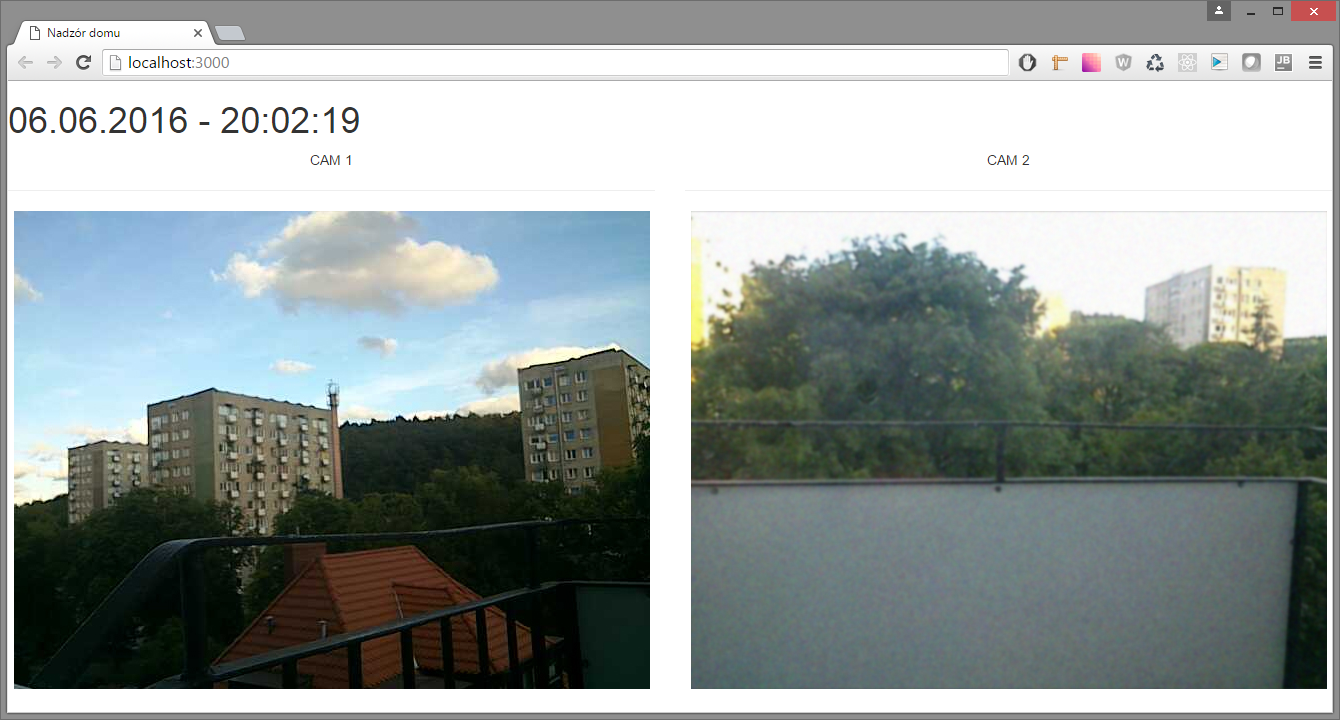
\includegraphics[width=12cm]{m_cam}
\caption{Działający system monitoringu. Opracowanie własne.}
\label{fig:cam}
\end{figure} 

Niskie tempo odświeżania rekompensuje fakt, iż możemy podłączyć wiele kamer i mieć odczyt na żywo z każdej z nich. W naszym przypadku całkowicie zerowym kosztem stworzyliśmy system nadzoru domu, do którego można się zalogować. Do zabezpieczenia aplikacji użyliśmy standardowej autoryzacji poprzez HTTP, której obsługę do Meteora dodaliśmy przy pomocy modułu Jabbslad/basic-auth.

\section{Budowa inteligetnego oswietlenia}


% zakończenie
\summary
Stworzenie systemu monitoringu pozwoliło mi lepiej poznać Node.js oraz samego Meteora. Pomimo, że aplikacja jest bardzo prosta w założeniach poświęciłem mnóstwo czasu na szukanie informacji w internecie jak rozwiązywać kolejno napotykane problemy. Jednak tak jak pisałem w ostatnim rozdziale takie udogodnienia niosą za sobą spore ryzyko. O ile my naszą aplikację zabezpieczyliśmy najprostszym i najskuteczniejszym sposobem, być może w przyszłości będziemy chcieli prowadzić logowanie wielu użytkowników co może wprowadzić lukę dla hackera. Jednak z drugiej strony warto korzystać z technologii aby ułatwić sobie życie w każdym możliwym aspekcie. 
Uważam, że wybrane do tej części projektu technologie idealnie sprawdzają się do naszych zastosowań. Node.js jest bardzo szybki w porównaniu do starszych technologii i idealnie sprawdza się w naszym zastosowaniu.

% załączniki (opcjonalnie):
\appendix

% literatura (obowiązkowo):
\bibliographystyle{unsrt}
\bibliography{xml}

% spis tabel (jeżeli jest potrzebny):
%\listoftables

% spis rysunków (jeżeli jest potrzebny):
\listoffigures

\oswiadczenie

\end{document}